% national A q19 fig1: five-hedron schematic projection
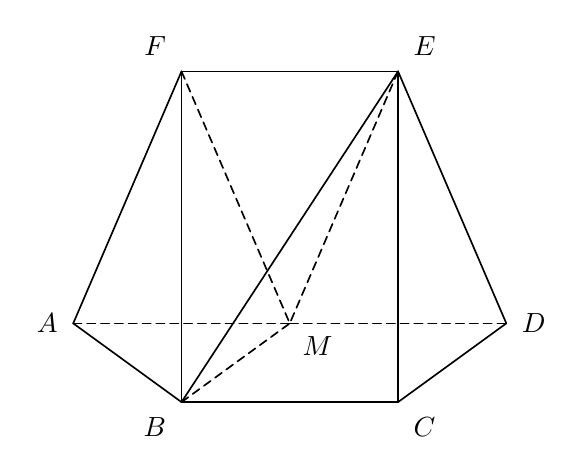
\begin{tikzpicture}[line width=.6pt, line join=round, line cap=round]
\coordinate (A) at (0,1);
\coordinate (B) at (1.3750000000,0.0000000000);
\coordinate (C) at (4.1250000000,0.0000000000);
\coordinate (D) at (5.5,1);
\coordinate (M) at (2.75,1);
\coordinate (F) at (1.3750000000,4.2000000000);
\coordinate (E) at (4.1250000000,4.2000000000);
% solid outer / front
\draw[solid] (F) -- (E);
\draw[solid] (F) -- (A);
\draw[solid] (E) -- (D);
\draw[solid] (A) -- (B);
\draw[solid] (B) -- (C);
\draw[solid] (C) -- (D);
% solid inner diagonals
\draw[solid] (F) -- (B);
\draw[solid] (B) -- (E);
\draw[solid] (C) -- (E);
% dashed hidden
\draw[densely dashed] (A) -- (M);
\draw[densely dashed] (M) -- (D);
\draw[densely dashed] (B) -- (M);
\draw[densely dashed] (F) -- (M);
\draw[densely dashed] (E) -- (M);
% labels offset from strokes
\node[above left=2pt] at (F) {$F$};
\node[above right=2pt] at (E) {$E$};
\node[left=2pt] at (A) {$A$};
\node[below left=2pt] at (B) {$B$};
\node[below right=2pt] at (C) {$C$};
\node[right=2pt] at (D) {$D$};
\node[below right=2pt,xshift=-1.0pt,yshift=1.0pt] at (M) {$M$};
\end{tikzpicture}
